 % Utilisez la macro de langue appropriée.
 % Noter que toutes les parties du document,
 % à part les articles, doivent être en français.
 % Pour rédiger une thèse en anglais, il faut
 % une permission. Consulter le guide de présentation
 % des mémoires et des thèses pour de l'information
 % plus détaillé et à jour.
%%\francais   %ou
\anglais
\chapter*{Introduction}

\section{A case for tools and methods}

The way that species interact with one another provides a `point of
departure' from which to study or understand biodiversity and the
environment at a range of scales \cite{Jordano2016ChaEco}. Ranging from
understanding how interactions can shape and drive population dynamics,
the maintenance and functioning of ecosystems, as well as long-term
evolutionary dynamics \cite{Landi2018ComSta, Albrecht2018PlaAni}.
Species interactions (and the resulting networks) can be formalised
and viewed under the lens of graph theory \cite{Dale2010GraSpa} - with
species being nodes and interactions being edges. This provides us with
a robust framework built on a mathematical foundation from which to approach
network analysis and quantify various measures of network structure and
behaviour \cite{Delmas2019AnaEco}.

In the process of assembling ecological networks as graphs we are also
`encoding' an `ecological fingerprint' for that community. This raises
the question of how far we can take the the idea of `decoding' networks
by leveraging the mathematical framework to better understand the
information that they contain. In particular by leaning on the
mathematical properties (and the ecological information they represent)
to make network predictions, and as a means to provide us with more
information as to how networks may vary over time or spatial scales.

Although the field of network ecology might have a strong conceptual and
theoretical basis from which to work with we are still at somewhat of a
loss when is comes to our ability to leverage this framework to make any
generalised or macroecological conclusions about the properties of networks
over larger geographic scales (although see \cite{Baiser2019Ecogeographical, Pinheiro2023Latitudinal} who explicitly try and tie networks to classical macroecological theories/laws).
This limited understanding can (at least in a large part) be attributed to
the sparse global coverage of data \cite{Poisot2021GloKno, Cameron2019UneGlo},
which itself is driven by the immense
challenges associated with observing and recording interactions in the field 
\cite{Bennett2019PotPit, Jordano2016SamNet}. Given the limited feasibility
of being able to curate interaction datasets in a way that will result in
a global coverage it makes sense to turn to predictive methods as a way to
begin filling in the 'gaps' of the global map of interaction data. Although
this may seem a daunting task we can lean on the mathematical formalisation
and the information that networks contain to make this a possibility, once
we have crossed that bridge we may then find ourselves in a position to be
able to ask more global-minded questions.

This pipeline from prediction to global questions is shown in \autoref{fig:plan}
and is the mainstay of this thesis document \emph{i.e.,} the thesis itself
can be thought of as two parts. The first part is addressing
the need for predictive tools and discussing as well as developing methods we
can use to begin filling in the global map. The second phase of the thesis briefly touches on some new 'tools' we can use when we start to think about large scale questions pertaining to network properties, specifically
the question of network complexity and how the definition thereof matters, as well
as network boundaries.

\begin{figure}[h]
    \centering
    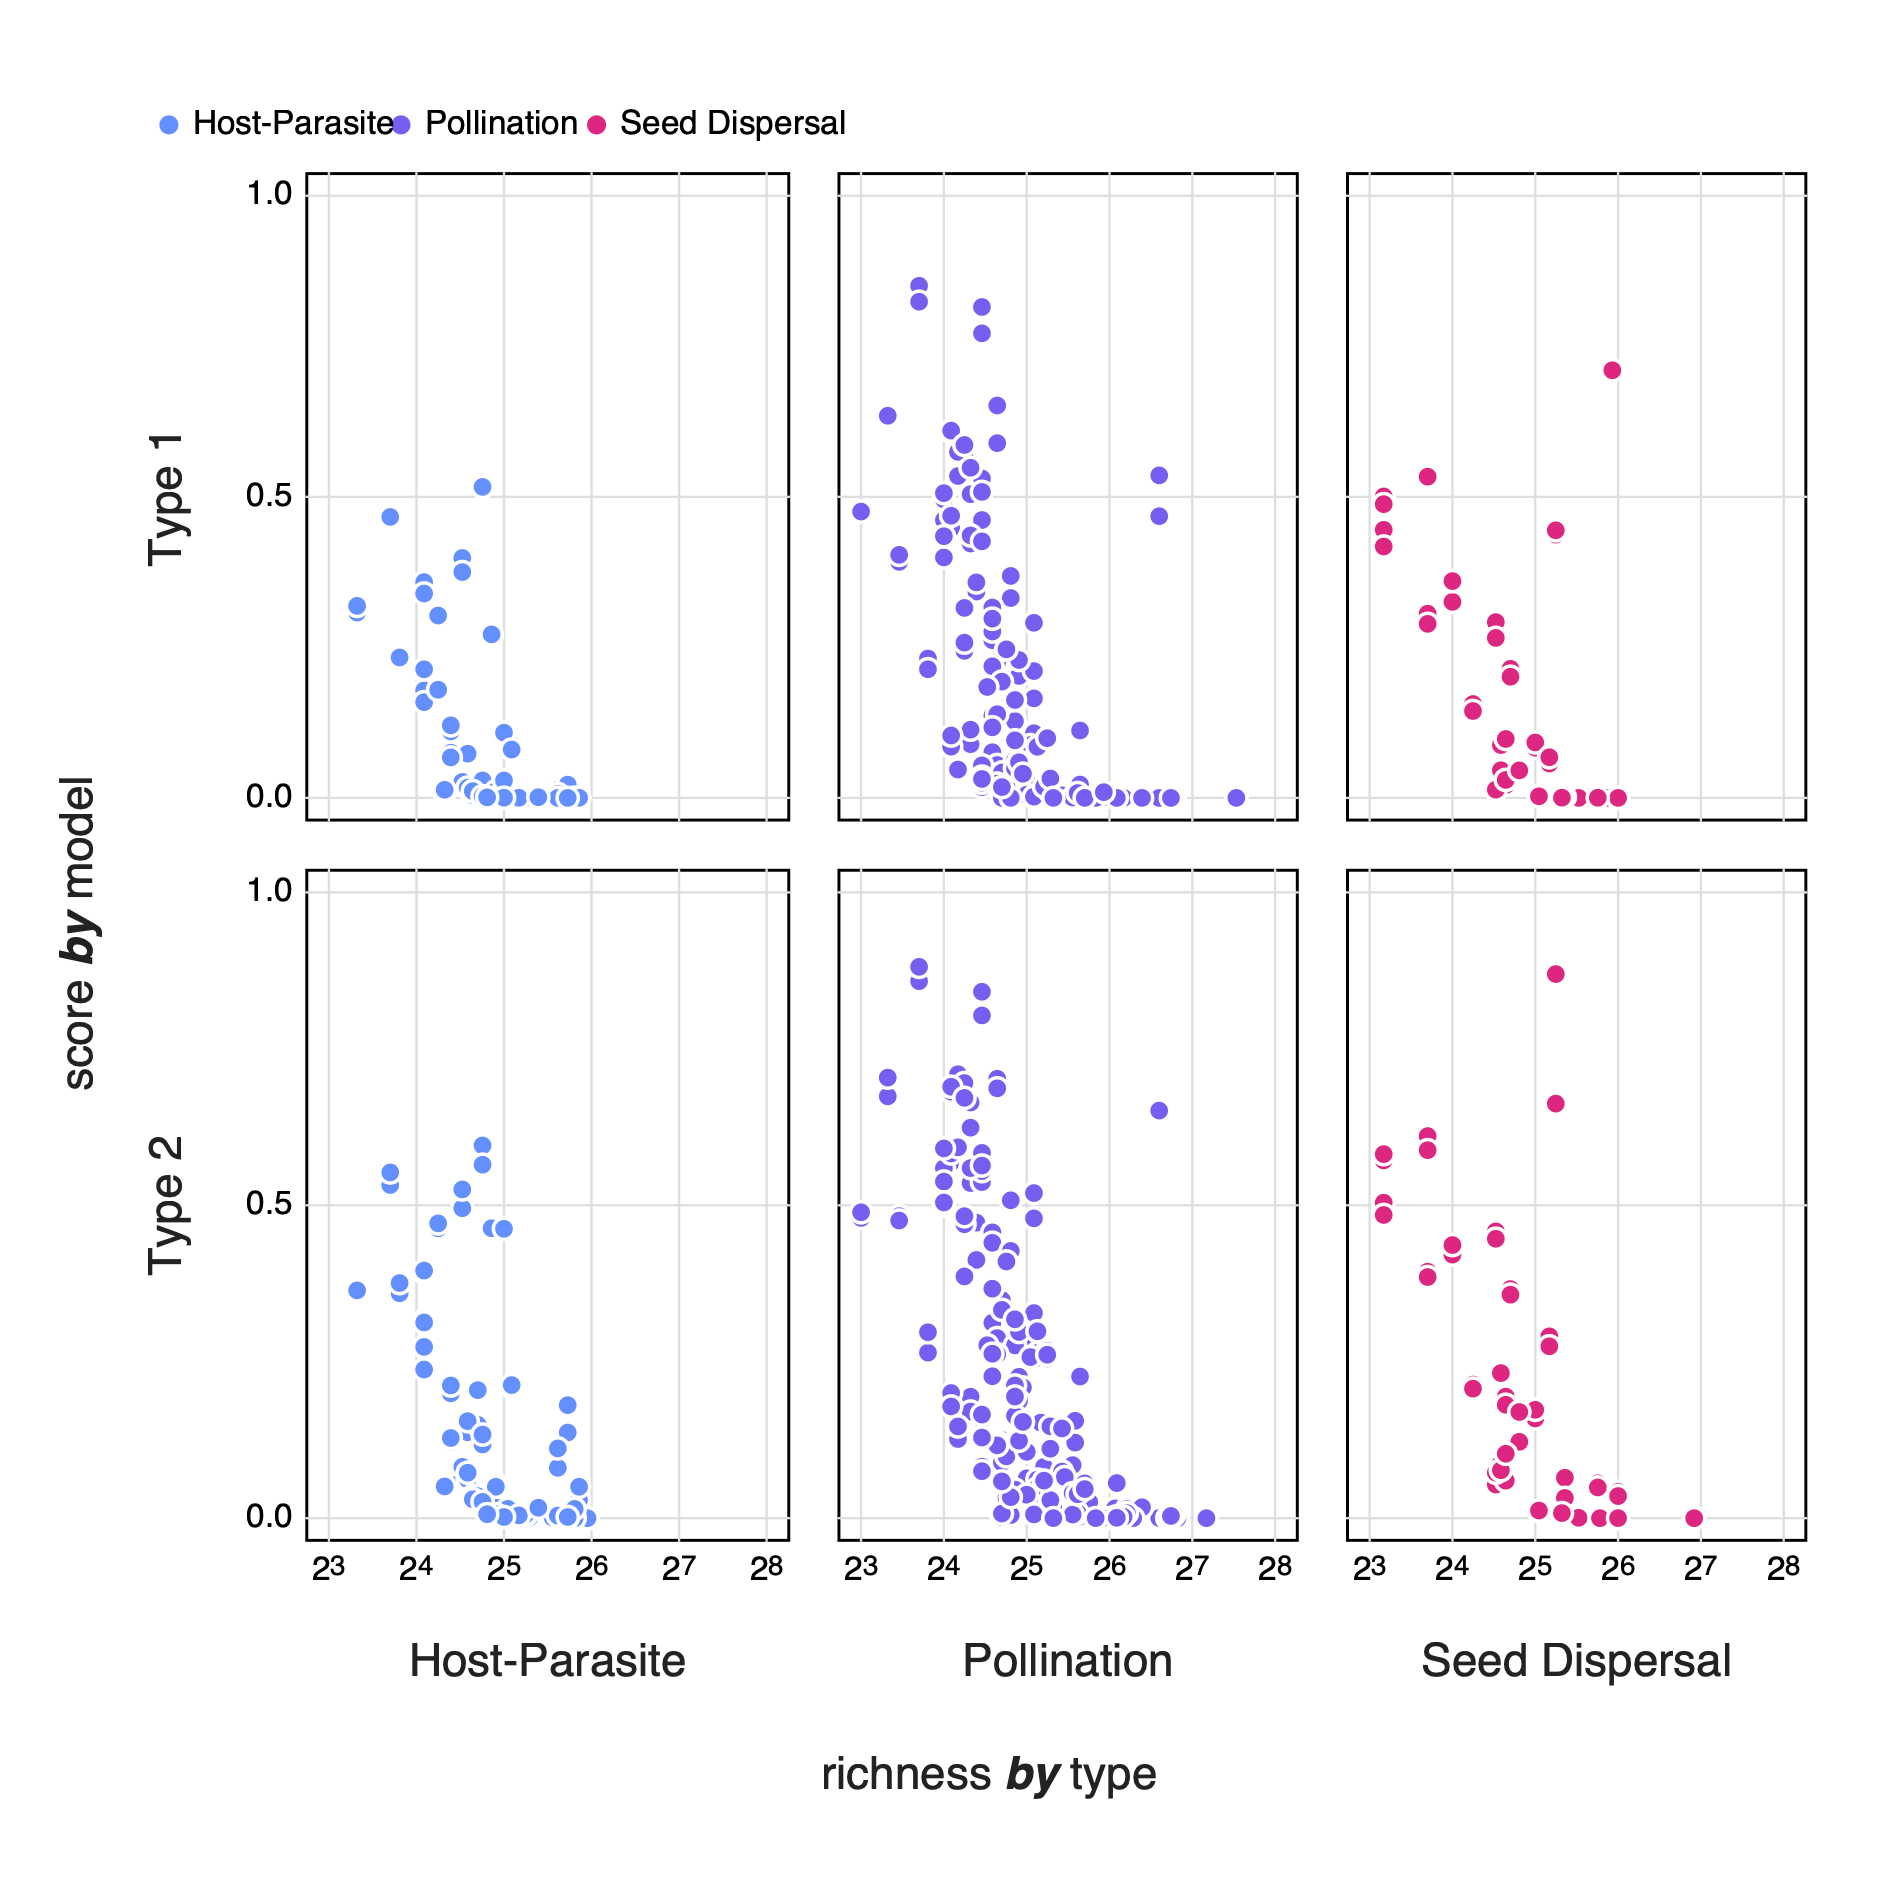
\includegraphics[width=\textwidth]{figures/nullmodel_richness.png}
    \caption{One of the biggest factors limiting our ability to ask global questions about ecological networks is the lack of global data. This figure provides a high-level overview of how the development and adoption of predictive methods will equip us to begin asking and answering large-scale questions. Two of these 'global questions' that are asked in this thesis are shown}
    \label{fig:plan}
\end{figure}

\subsection{Prediction for gap-filling}

Current methods are often conceptualised around and focused on a single facet of the
larger process at play such phylogenetic matching
\cite{Pomeranz2018InfPre, Elmasri2020HieBay}, or functional traits
\cite{Bartomeus2016ComFra}. Although recent applications of ensemble
modelling \cite{Becker2020PreWil}, and discussions on the potential of
machine learning methods \cite{Desjardins-Proulx2019ArtInt} show promise
in addressing methodological constraints to prediction and the growth of
open tools and data may mitigate some data constraints in the coming
years. However, we still lack a clear path forward or research agenda as
to how we can maximise and integrate these resources.

The task of trying to predict networks is discussed in chapters \ref{Roadmap}
and \ref{Perspectives}, where my collaborators and myself map out and
discuss the the methodological considerations when trying to approach the task
of network prediction. Chapter~\ref{Roadmap} provides a more scoping discussion
on these methods, whereas Chapter~\ref{Perspectives} represents a more detailed
discussion on the prospect of using graph embedding and transfer learning
for network prediction. These specific methods are also the framework presented
and used in Chapter~\ref{Foodweb}. This section acts as a 'proof-of-concept'
showcasing that the task of network prediction is both attainable and
capable of producing ecologically plausible networks.

\subsection{From prediction to global patterns}

Although prediction is a powerful tool in the immediate/local sense 
(\emph{e.g.,} it can allow local land managers/custodians to have a 
first approximation
of how species may be interacting in that given area it is of course
also a possible what to fill in the global map. A 'filled map' will
allow us to be poised to develop a more mechanistic, global scaled,
understanding of networks. The work presented in this thesis represents
but a tentative and small initial foray in this direction. Namely
Chapter~\ref{SVD}, which presents a different, more information theory 
approach to defining complexity using the singular value vector component
of an SVD \cite{Shannon1948MatThe}. The final chapter of this thesis
(Chapter~\ref{SpatialBoundaries}) is a \texttt{Julia} package that
allows users to implement the Wombling algorithm (an edge
detection mechanism; \cite{Womble1951DifSys}).

Wombling has been discussed as a useful tool for spatial analyses in
ecology \cite{Fortin2005SpaAna} and has been used to detect transitions
across a landscape \cite{Philibert2008SpaStr}, changes in biological
variables in communities \cite{Barbujani1989DetReg} and to analyse the
spread of invasive species \cite{Fitzpatrick2010EcoBou}. Being able to
subdivide networks into patches within a landscape will help us better
understand the boundaries of and between networks as well as how these
may relate to species or community changes and boundaries - such as when
transitioning across habitat `boundaries' \cite{Hackett2019ResOur}.

\subsection{Objectives}\label{objectives-and-hypotheses}

Being able to understand, quantify, and work with ecological networks is
important from a conservation and land management perspective as this
will have cascading implications with regards to ecosystem functioning
and stability. Yet we are severely hamstrung by a lack of high-quality,
usable data as well as an appropriate set of tools that can be used to
contextualise and understand ecological networks. There is a need for
tools that can help us construct networks for where there are no data
\emph{i.e.,} make predictions as well as developing tools (or ideas) that
can be used to help further our mechanistic understanding of networks once
we are at a point where we have the large scale data to do so. My work will
help address these two issues in the context of developing tools that will
either directly enable us to make predictions (Chapters~\ref{Roadmap},
\ref{Perspectives}, and \ref{Foodweb}), or present methods that are aligned
with global (large-scale) questions that will allow us to compare networks
(Chapter~\ref{SVD}) or attempt to delineate them 
(Chapter~\ref{SpatialBoundaries}).

\section{Methodological overview}

\subsection{Contemplation and consideration}

In the following sections I will break these ideas and questions down
further, focusing on how we can access (decode) the information in
networks, and how this can be used to inform us on the amount of
information contained in networks as well as as the applicability within
the context of network prediction - with the specific aim of
constructing the Canadian metaweb. Once we have the ability to predict
networks we are then poised to begin approaching detecting boundaries
\emph{i.e.} changes between networks across space. Broadly this will
address two areas of which we currently have a gap within network
ecology \emph{i}) overcoming the issue of lack of empirical data of
networks \cite{Poisot2021GloKno} through prediction and \emph{ii})
beginning an initial foray into understanding the variation of networks
over space - another aspect of network ecology that is still in its
infancy (although see \cite{Fortin2021NetEcoa} for a discussion of the
possibilities of this direction of study).

\subsection{Transfer learning for network prediction}

Transfer learning is a machine learning methodology that uses the 
knowledge gained when solving a known problem and
applying it to solve a (related) problem by transferring the knowledge
across a shared medium (space) \cite{Torrey2010TraLea, Pan2010SurTra}.
The concept of transfer learning is
an approach that is particularly well suited for the problem of network
prediction as it allows us to lean on the data that are available to 
enable us to make \emph{de novo} predictions. This could be as simple
as pinpointing missing interactions in the existing data 
(\emph{e.g.,} pairwise learning has been used to predict plant-pollinator
interactions in \cite{Stock2021PaiLea}) as well as a way to predict
novel interactions (\emph{i.e.,} fill in those global gaps). This,
in a sense allows us to bring knowledge with us from an area for
which we \emph{have} data to an area where it is \emph{lacking}. In the
case of predicting species interactions transfer learning as an idea 
works because interactions are being conserved at an evolutionary scale using
phylogenetic relatedness for a given community can inform as how they
interact with each other \cite{Davies2021EcoRed, Elmasri2020HieBay,
Gomez2010EcoInt}. Chapter~\ref{Foodweb} presents a transfer learning framework
and uses the task of constructing a Canadian metaweb using the European metaweb
assembled by \cite{Maiorano2020TetSpe} as a proof-of-concept the workflow and
data itself can be found \href{https://osf.io/2zwqm/}{here}. Below is a
high-level summary of that framework.

\subsubsection{Learning using graph embedding}

Before one can transfer any knowledge we must first learn something about
the system using known data. Since ecological networks can be represented
by their adjacency matrices we can turn to graph theory to help us find a
way to learn something about the known interaction network. Graph embedding
is a low dimensional representation of the graph but, importantly, still
preserves its topology \cite{Yan2005Graph}. This process essentially allows
as to learn something about where species (nodes) are situated within the
network - which (in an abstract way) informs us of the the role a species
plays in the community. There are multiple embedding approaches discussed
in Chapter~\ref{Perspectives}, but in the context of the framework developed
in Chapter~\ref{Foodweb} we will focus on the use of SVD as an embedding 
technique. SVD presents an appropriate embedding of ecological networks, having
been shown to both capture their complex, emerging properties
\cite{Strydom2021SvdEnt} and allow for the highly accurate prediction
of the interactions within a single network \cite{Poisot2021ImpMam}.

\subsubsection{Graph embedding using SVD}

Singular Value Decomposition \cite{Forsythe1967ComSol, Golub1971SinVal} 
is the factorisation of an adjacency matrix \(\mathbf{A}\) (where
\(\mathbf{A}_{m,n} \in\mathbb{B}\)) into the form:

\[ \mathbf{U}\cdot\mathbf{\Sigma}\cdot\mathbf{V}^T \]

Where \(\mathbf{U}\) is an \(m \times m\) orthogonal matrix and
\(\mathbf{V}\) an \(n \times n\) orthogonal matrix. The columns in these
matrices are, respectively, the left- and right-singular vectors of
\(\mathbf{A}\). \(\mathbf{\Sigma}\) is a diagonal matrix that contains
only non-negative \(\sigma\) values. Where \(\sigma_{i} = \Sigma{ii}\),
and contains the singular values of \(\mathbf{A}\).
 
An SVD can be truncated so as to remove additional noise in the dataset by
omitting non-zero and/or smaller \(\sigma\) values from
\(\mathbf{\Sigma}\) using the rank of the matrix. Under a t-SVD
\(\mathbf{A}_{m,n}\) is decomposed so that \(\mathbf{\Sigma}\) is a
square \(r \times r\) diagonal matrix (whith \(1 \le r \le r_{full}\)
where \(r_{full}\) is the full rank of \(\mathbf{A}\) and \(r\) the rank
at which we truncate the matrix). Additionally, \(\mathbf{U}_{t}\) is now a
\(m \times r\) semi unitary matrix and \(\mathbf{V}'_{t}\) a \(n \times r\)
semi-unitary matrix.

In the context of 'learning using embedding' the learned information is
captured using an SVD, however for the task of network prediction we modified
the products of the SVD so that they could be used for an RDPG. An RDPG 
estimates the probability of observing interactions between
nodes (species) as a function of the nodes' latent variables, and is a
way to turn an SVD (which decompose one matrix into three) into two
matrices that can be multiplied to provide an approximation of the
network. The latent variables used for the RDPG, called the left and
right subspaces, are defined as
$\mathscr{L} = \mathbf{U}\sqrt{\mathbf{\Sigma}}$, and
$\mathscr{R} = \sqrt{\mathbf{\Sigma}}\mathbf{V}'$ -- using the full
rank of $\mathbf{A}, \mathscr{L}\mathscr{R} = \mathbf{A}$, and
using any smaller rank results in
$\mathscr{L}\mathscr{R} \approx \mathbf{A}$. 
(hereafter referred to the left ($\hat{\mathscr{L}}$) and right 
($\hat{\mathscr{R}}$) subspaces respectively). These
subspaces are ecologically informative and tell us about the 'generality'
(think predator capacity, \emph{sensu} \cite{Schoener1989Food}) and 
'vulnerability' (think capacity to be prey, \emph{sensu} \cite{Schoener1989Food})
of the species in the European network. This in essence provides us with
an idea of where a species is likely to occur within a network/the space
it occupies in the network.

\subsubsection{Transferring and inferring using phylogenetic relatedness}

In order to transfer the knowledge (the generality and vulnerability
values) from the European metaweb to the
Canadian species pool, we performed ancestral character estimation using
a Brownian motion model and the Upham \cite{Upham2019InfMam} mammalian
phylogeny. This uses the estimated
feature vectors (left and right subspaces) for the European mammals to
create a state reconstruction for all species and allows us to impute
the missing generality and vulnerability values for the Canadian
species that are not already in the European network. Essentially this
allows us to infer where in the two subspaces the Canadian mammals are
located.

\subsubsection{Novel Prediction using RDPG}

AS we now essentially have the left and right subspaces for the Canadian
metaweb we can directly multiply these to yield the metaweb, specifically
using an RDPG. The phylogenetic reconstruction of ($\hat{\mathscr{L}}$) and
($\hat{\mathscr{R}}$) has an associated uncertainty, therefore, we can
assemble a \emph{probabilistic} metaweb in \emph{sensu} \cite{Poisot2016StrPro},
\emph{i.e.} in which every interaction is represented as a single,
independent, Bernoulli event of probability \(p\).

\subsection{SVD entropy: a measure of network
complexity}\label{svd-entropy-a-measure-of-network-complexity}

Singular value decomposition also offers two interesting candidate measures
of complexity for ecological networks. The first measure is the rank of
the matrix. The rank of $\mathbf{A}$ (noted as
$r = \text{rk}(\mathbf{A})$) is the dimension of the vector space
spanned by the matrix and corresponds to the number of linearly
independent rows or columns, which works as an estimate of `external
complexity', in that it describes the dimension of the vector space of
the matrix, and therefore the number of linearly independent rows (or
columns) of it. From an ecological standpoint, this quantifies the
number of unique `strategies' represented in the network.

The second measure is to calculate the entropy of the matrix obtained
through SVD by using the singular values \cite{@Shannon1948MatThe}. This
so-called SVD entropy measures the extent to which each rank encodes an
equal amount of information, as the singular values capture the
importance of each rank to reconstruct the original matrix; this
approach therefore serves as a measure of `internal complexity'.

Intuitively, the singular value $i$ ($\sigma_i$) measures how much
of the dataset is (proportionally) explained by each vector - therefore,
one can measure the entropy of \(\mathbf{\sigma}\) following
\cite{Shannon1948MatThe}. High values of SVD entropy reflects that all vectors
are equally important, \emph{i.e.} that the structure of the ecological
network cannot efficiently be compressed, and therefore indicates high
complexity \cite{Gu2016HowLon}. Because networks have different
dimensions, we can use Pielou's evenness \cite{Pielou1975EcoDiv} to
ensure that values are lower than unity, and quantify SVD entropy, using
$s_i = \sigma_i/\text{sum}(\sigma)$ as:

$$J = -\frac{1}{\ln(k)}\sum_{i=1}^k s_i\cdot\ln(s_i)$$

Where \(k = \text{rk}(\mathbf{A})\) \emph{i.e.} the rank of the matrix,
which is equal to the number of non-zero entries in \(\mathbf{\Sigma}\)
as per the Eckart-Young-Mirsky theorem \cite{Eckart1936AppOne,
Golub1987GenEck}. 

We used all bipartite networks contained in the \texttt{web-of-life.es}
database and measured both their external (rank) and internal (SVD entropy)
complexity. As this database extracted species interaction networks from
supplementary materials across all inhabited continents and covers a large range
of sampling years, environments, organisms, and sampling methodologies. As such,
this dataset is particularly suited to describe the general trends across
\emph{global} ecological networks.

\subsection{Spatial wombling for edge detection}

Spatial wombling (an edge detection algorithm; \cite{Womble1951DifSys}) could
prove to be a promising approach to trying to detect boundaries between
networks. Chapter~\ref{SpatialBoundaries} presents a \texttt{Julia} package that
implements both the lattice and triangulation wombling algorithms. 

Broadly, wombling interpolates between a given set of points.
Two core metrics that are derived by this process is the rate of change
\(m\) which is calculated as:

$$m = \sqrt{\frac{\partial f(x,y)}{\partial x}^2 + \frac{\partial
f(x,y)}{\partial y}^2}$$

This can be used to find the zones (or cells) of rapid change across the
landscape and identify potential candidate boundaries. It is also
possible to calculate the direction (\(\theta\)) for each rate of
change. This is calculated as:

$$\theta = \arctan \left( \frac{\partial f(x,y)}{\partial y} \bigg/ \frac{\partial f(x,y)}{\partial x} \right) + \Delta$$

$$\text{where} \quad \Delta =
\left\{ \begin{array}{ccc}
    0 \degree & \text{if} & \frac{\partial f(x,y)}{\partial x} \geq 0 \\
    180 \degree & \text{if} & \frac{\partial f(x,y)}{\partial x} < 0 \\
\end{array} \right\}$$

Both $m$ and $\theta$ are an approximation on the `topology' of a
certain metric ($z$, \emph{e.g.} number of species) between a
collection of points. Similarity between the $z$ values indicates a
uniformity between those points and thus a low rate of change where as a
high degree of difference for the given window is indicative of rapid
change \emph{i.e.} a boundary as we transition from one zone to the
next.

\subsubsection{Lattice wombling}

For a lattice of points where one will have sampling locations arranged
uniformly across space one can simply use the co-ordinates 'as is' and 
$f(x,y)$ can be calculated as:

$$f(x,y) = z_{1}(1-x)(1-y) + z_{2}x(1-y) + z_{3}x y + z_{4}(1-x)y$$

For convenience the centroid of the square \emph{i.e.} the values of
$x$ and $y$ can be standardised to 0.5. 

\subsubsection{Triangulation wombling}

When working with points that are irregularly distributed across the 
landscape it is possible to use triangulation wombling 
\cite{Fortin1995DelEco}. The three nearest
neighbours can be determined using a Delaunay triangulation algorithm
\cite{Delaunay1934SphVid} and $f(x,y)$ can be calculated as:

$$f(x,y) = ax + by + c$$

where:

$$ \left[ \begin{array}{ccc} a & b & c \end{array} \right] = 
\left[ {\begin{array}{ccc}
   x_{1} & y_{1} & 1\\
   x_{2} & y_{2} & 1\\
   x_{3} & y_{3} & 1\\
  \end{array} } \right]^{-1}\cdot
  \left[
  \begin{array}{ccc} z_{1} & z_{2} & z_{3} \end{array} \right]$$

and the position of the centroid being calculated as:

$$ \Big( \frac{x_{1} + x_{2} + x_{3}}{3} \Big), \Big( \frac{y_{1} + y_{2} +
y_{3}}{3} \Big) $$

\subsubsection{Boundary detection}

Detecting boundaries \emph{i.e.} areas where the angle of the landscape
transitions sharply is surprisingly simple. After having calculated the
rate of change (\(m\)) for the geographical area it is possible to use
these values to identify and assign potential boundaries
\cite{Fortin2005SpaAna, Oden1993CatWom, Fortin1995DelEco}. Following the
approach outlined in \cite{Fortin2005SpaAna} a threshold value (or
percentile class) can be set and will determine what proportion of cells
will be retained as potential boundaries. For example if using a 0.1
threshold then the highest 10\% of points (which are ranked based on 
\(m\)) will be classified as candidate boundaries.

\section{Chapter summaries}

\subsection{Chapter 1: A roadmap for predicting ecological networks}

\cite{Strydom2021RoaPre} (as the name suggests) maps out a series of questions
and considerations with regards to approaching the challenge of
predicting species interactions across space and time. Points of
discussion regarding predicting network structure and interactions
include the value of the simultaneous prediction of occurrence and
interactions (\emph{e.g.} \cite{Zurell2020TesSpe}, why connectance
as a useful property to use for predictions and dealing with 
potentially novel interactions.

\subsection{Chapter 2: Graph embedding for network prediction}

This chapter should be viewed as a companion piece for Chapter~\ref{Foodweb}
as it provides larger conceptual discussions around the potential
applications of graph embedding and how these relate to transfer
learning. In addition to the more methodological discussions we
also delve into the applications of prediction and how this should
be done in a way that does 'no harm'. This section also includes
what could be considered some vital discussions on how we can
advance the way we think about and define the original definition
of a 'metaweb' \emph{sensu} \cite{Dunne2006NetStr}.

\subsection{Chapter 3: Prediction in action: The Canadian
Metaweb}

Building on the ideas in \cite{Strydom2021RoaPre}, work on the use of 
transfer learning for predicting \emph{de novo} interactions
\cite{Runghen2021ExpNod}, and the applicability of phylogenetic
reconstruction within the context of ecological networks \emph{e.g.,}
\cite{Braga2021PhyRec}, we set out to create a probabilistic metaweb for
terrestrial Canadian mammals in \cite{Strydom2021FooWeb}. What is 
perhaps most exciting about this chapter is that despite sharing about
only 4\% of species between Canada and Europe
we were able to construct a metaweb that correctly predicted about 91\%
of the species interactions in Canada (this was achieved by using known
datasets to validate predicted interactions), which speaks to the
`robustness' of this transfer learning framework and potential
applicability in a variety of settings (\emph{e.g.,} as an `informative prior'
from which more localised/spatially explicit networks can be constructed
\cite{Cirtwill2019QuaFra}) to help in filling in the blank
spaces on the map when it comes to regional food webs.

\subsection{Chapter 4: SVD entropy: a measure of network complexity}

In \cite{Strydom2021SvdEnt} we present SVD entropy as a starting point to
unifying (and standardising) how we define the complexity of ecological
networks. We argue that having a unified definition will allow us to
revisit how complexity relates to the ecological properties of networks
using a standardised framework that focuses on the physical complexity
of networks as opposed to the complexity of the behaviour of the system.
An interesting result from using SVD entropy is that the complexity of
ecological networks is indeed \emph{immense}, yet despite this high
complexity networks are still not reaching their \emph{maximum}
potential complexity, which raises questions for future contemplation
with regards to understanding what might be constraining network
complexity. An additional observation is that the relationship between 
network size, connectance and complexity. Results
point to the potential constraint of network size on complexity.
Networks at the early assembly stages tend to be severely constrained
\cite{Barbier2018GenAss, Saravia2018EcoNet} due to conditions needed
for the persistence of multiple species. As networks grow larger, these
constraints may ``relax'', leading in networks with more redundancy, and
therefore a lower complexity.

\subsection{Chapter 5: SpatialBoundaries.jl: a software for boundary detection}

Here we present a \texttt{Julia} package, (the documentation is available
\href{https://poisotlab.github.io/SpatialBoundaries.jl/dev/}{here})
that has the functionality to implement the spatial wombling algorithm
across both a uniform landscape \emph{i.e.} lattice wombling as well as
irregular/random landscapes \emph{i.e.} triangulation wombling. These
two methods still calculate the rate of change (\(m\)) and
directionality (\(\theta\)) in the same manner but differ in how the
aggregate and quantify the surface for a set of points
\cite{Fortin2005SpaAna}. These are the two algorithms implemented in the
\texttt{SpatialBoundaries.jl} package, and should provide functionality
for most use cases when data are quantitative. \texttt{SpatialBoundaries.jl} 
has also been developed so as to integrate with other packages such as
\texttt{SimpleSDMLayers.jl}.

\section{Conclusion}\label{conclusion}

As a whole this thesis should be viewed as a computational toolbox for
network ecology that addresses both the issue of data scarcity through
the use of predictive tools (addressing the `Eltonian shortfall' highlighted by \cite{Hortal2015SevSho}) as well as presenting methods/ideas geared towards thinking about networks at global scales. This means that we would \emph{i}) have `tangible' networks from which we can begin to work with in various contexts or situations and \emph{ii}) have new methods/tools to begin asking questions about netwroks at a global scale. In other words adding more building blocks from which we can begin to take network ecology to the next level, \emph{i.e.,} bridging the gap from 'local-level network understanding' to 'tools for global netwrok analysis'.

\bibliographystyle{plain}
\sectionbibliography{ref_Intro.bib}

\endinput
%%
%% End of file `introduction.tex'.
